\documentclass[12pt, a4paper, oneside]{ctexart}
\usepackage{amsmath, amsthm, amssymb, bm, color, framed, graphicx, hyperref, mathrsfs, float}

% multi-column
\usepackage{tasks}
% itemize
\NewTasksEnvironment[label=(\arabic*), label-width=3ex]{exercise}

\everymath{\displaystyle}

\title{\textbf{第三次作业}}
\author{U08M11002 Spring 2022}
\date{提交截止日期:北京时间2022年3月28日}
\linespread{1}
\definecolor{shadecolor}{RGB}{241, 241, 255}

\newcounter{problemname}
\newenvironment{problem}{\stepcounter{problemname}\par\noindent\textbf{题目\arabic{problemname}. }}{\\\par}
\newenvironment{warning}{\begin{shaded}\par\noindent\textbf{提交作业方式:}}{\end{shaded}\par}

\begin{document}
	
	\maketitle
	
	\begin{warning}
		具体提交方式请以 QQ 群里助教的通知为准。
		\begin{enumerate}
			\item 为了你自己复习需要,\textbf{建议上交前自行扫描备份}。
		\end{enumerate}
	\end{warning}
	
	\hspace{1em}
	
	
	\begin{problem}
		描述某 LTI 系统的微分方程为 $y''(t) + 3 y'(t) + 2y(t) = 2f'(t) + 6 f(t)$,已知$y(0^-)=2$,$y'(0^-)=0$,$f(t)=U(t)$,求 $y(0^+)$ 和 $y'(0^+)$。
		\quad
	\end{problem}
	
	
	\begin{problem}
		对上题所描述的系统和起始条件,求该系统的零输入响应、零状态响应和全响应。
		\quad
	\end{problem}
	
	\begin{problem}
		上题所描述的系统,如果不知道起始条件,只知道初始条件$y(0^+)=3$,$y'(0^+)=1$,$f(t)=U(t)$,求该系统的零输入响应、零状态响应。
		\quad
	\end{problem}
	
	
	
	\begin{problem}
		描述某 LTI 系统的微分方程为 $y'(t) + 2 y(t) = f''(t) + f'(t) + 2f(t)$,若$f(t)=U(t)$,求该系统的零状态响应。
		\quad
	\end{problem}
	
	
	\begin{problem}
		已知某 LTI 系统的常微分方程为 $y'(t) + y(t) = f(t)$,
		\begin{exercise}(1)
			\task 若完全响应为$y(t)=[5e^{-t} + 3e^{-2t}]U(t)$,且$y(0^-)=5$,求该系统的零输入响应和零状态响应;
			\task 若$y(0^-)=10$,求系统的零输入响应;
			\task 若完全响应为$y(t)=[5e^{-t} + 3e^{-2t}]U(t)$,且$y(0^-)=5$,求$y'(t) + y(t) = f(t-2)$的零状态响应;
			\task 若完全响应为$y(t)=[5e^{-t} + 3e^{-2t}]U(t)$,且$y(0^-)=5$,求$y'(t) + y(t) = f'(t) + 2f(t)$的零状态响应。
		\end{exercise}
		\quad
	\end{problem}
	
	\begin{problem}
		已知描述系统的微分方程和起始状态如下,求零输入响应、零状态响应和全响应(从特征根求响应可以查表)。
		\begin{exercise}(1)
			\task $y''(t) + 4 y'(t) + 3y(t) =  f(t)$, $y(0^-)=1$,$y'(0^-)=1$,$f(t)=U(t)$
			\task $y''(t) + 4 y'(t) + 4y(t) =  f'(t) + 3 f(t)$, $y(0^-)=1$,$y'(0^-)=2$,$f(t)=e^{-t}U(t)$
			\task $y''(t) + 2 y'(t) + 2y(t) =  f'(t) $, $y(0^-)=0$,$y'(0^-)=1$,$f(t)=U(t)$
		\end{exercise}
		\quad
	\end{problem}
	
	\begin{problem}
		求上题中各系统的冲激响应。
		\quad
	\end{problem}
	
	\begin{problem}
		如下图所示电路,已知 $R=3\Omega$, $L=1H$, $C=0.5F$, $u_S(t)=\cos t U(t)V$, 求 $u_C(t)$ 的零状态响应。
		\begin{figure}[H]
			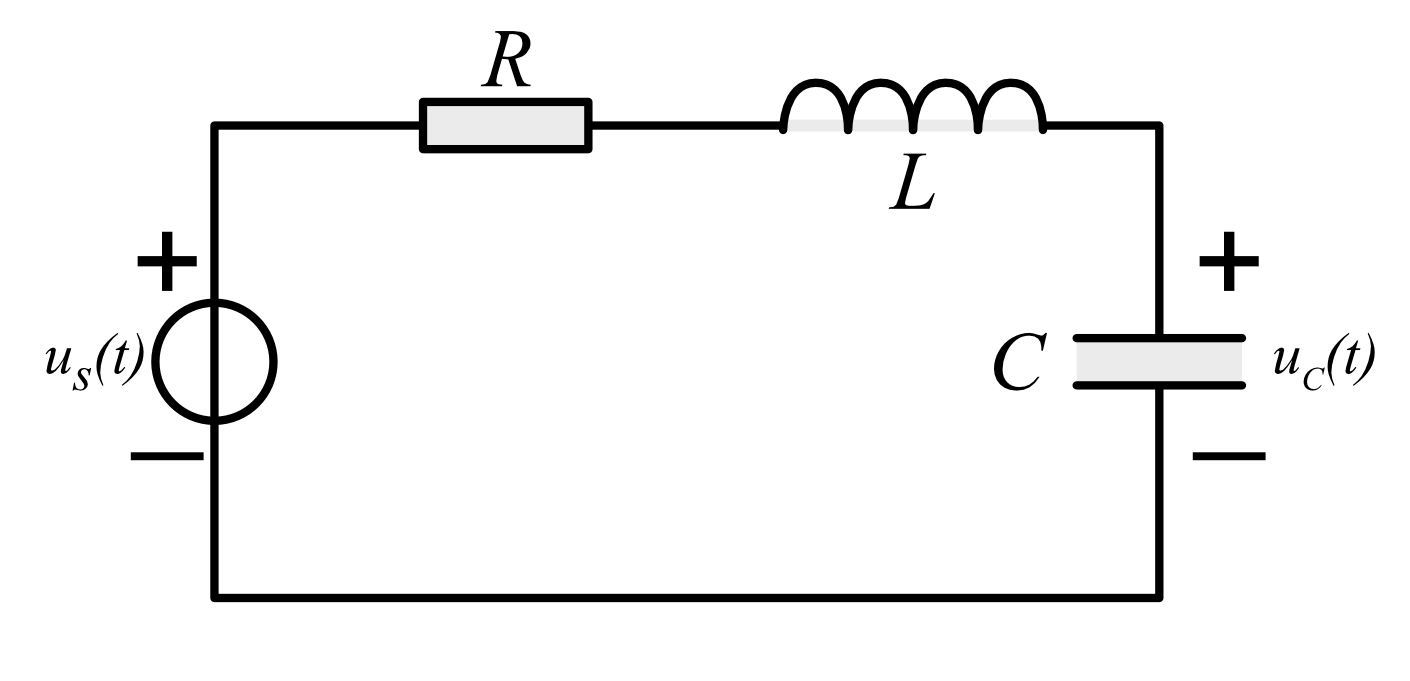
\includegraphics[width=8cm]{assets/hw3img2.png}
			\centering
		\end{figure}
		\quad
	\end{problem}
	
	
	\begin{problem}
		描述某二阶 LTI 系统的微分方程为 $y''(t) + 5y'(t) + 6y(t) = f(t)$,求冲激响应 $h(t)$。
		\quad
	\end{problem}
	
	\begin{problem}
		$f_1(t) = 3e^{-2t}U(t)$, $f_2(t) = 2U(t)$, $f_3(t) = 2U(t-2)$,求
		\begin{exercise}(2)
			\task $f_1(t) * f_2(t) $
			\task $f_1(t) * f_3(t) $
		\end{exercise}
		\quad
	\end{problem}
	
	\newpage
	
	\begin{problem}
		求下图中 $f_1(t)$ 和 $f_2(t)$ 的卷积。
		\begin{figure}[H]
			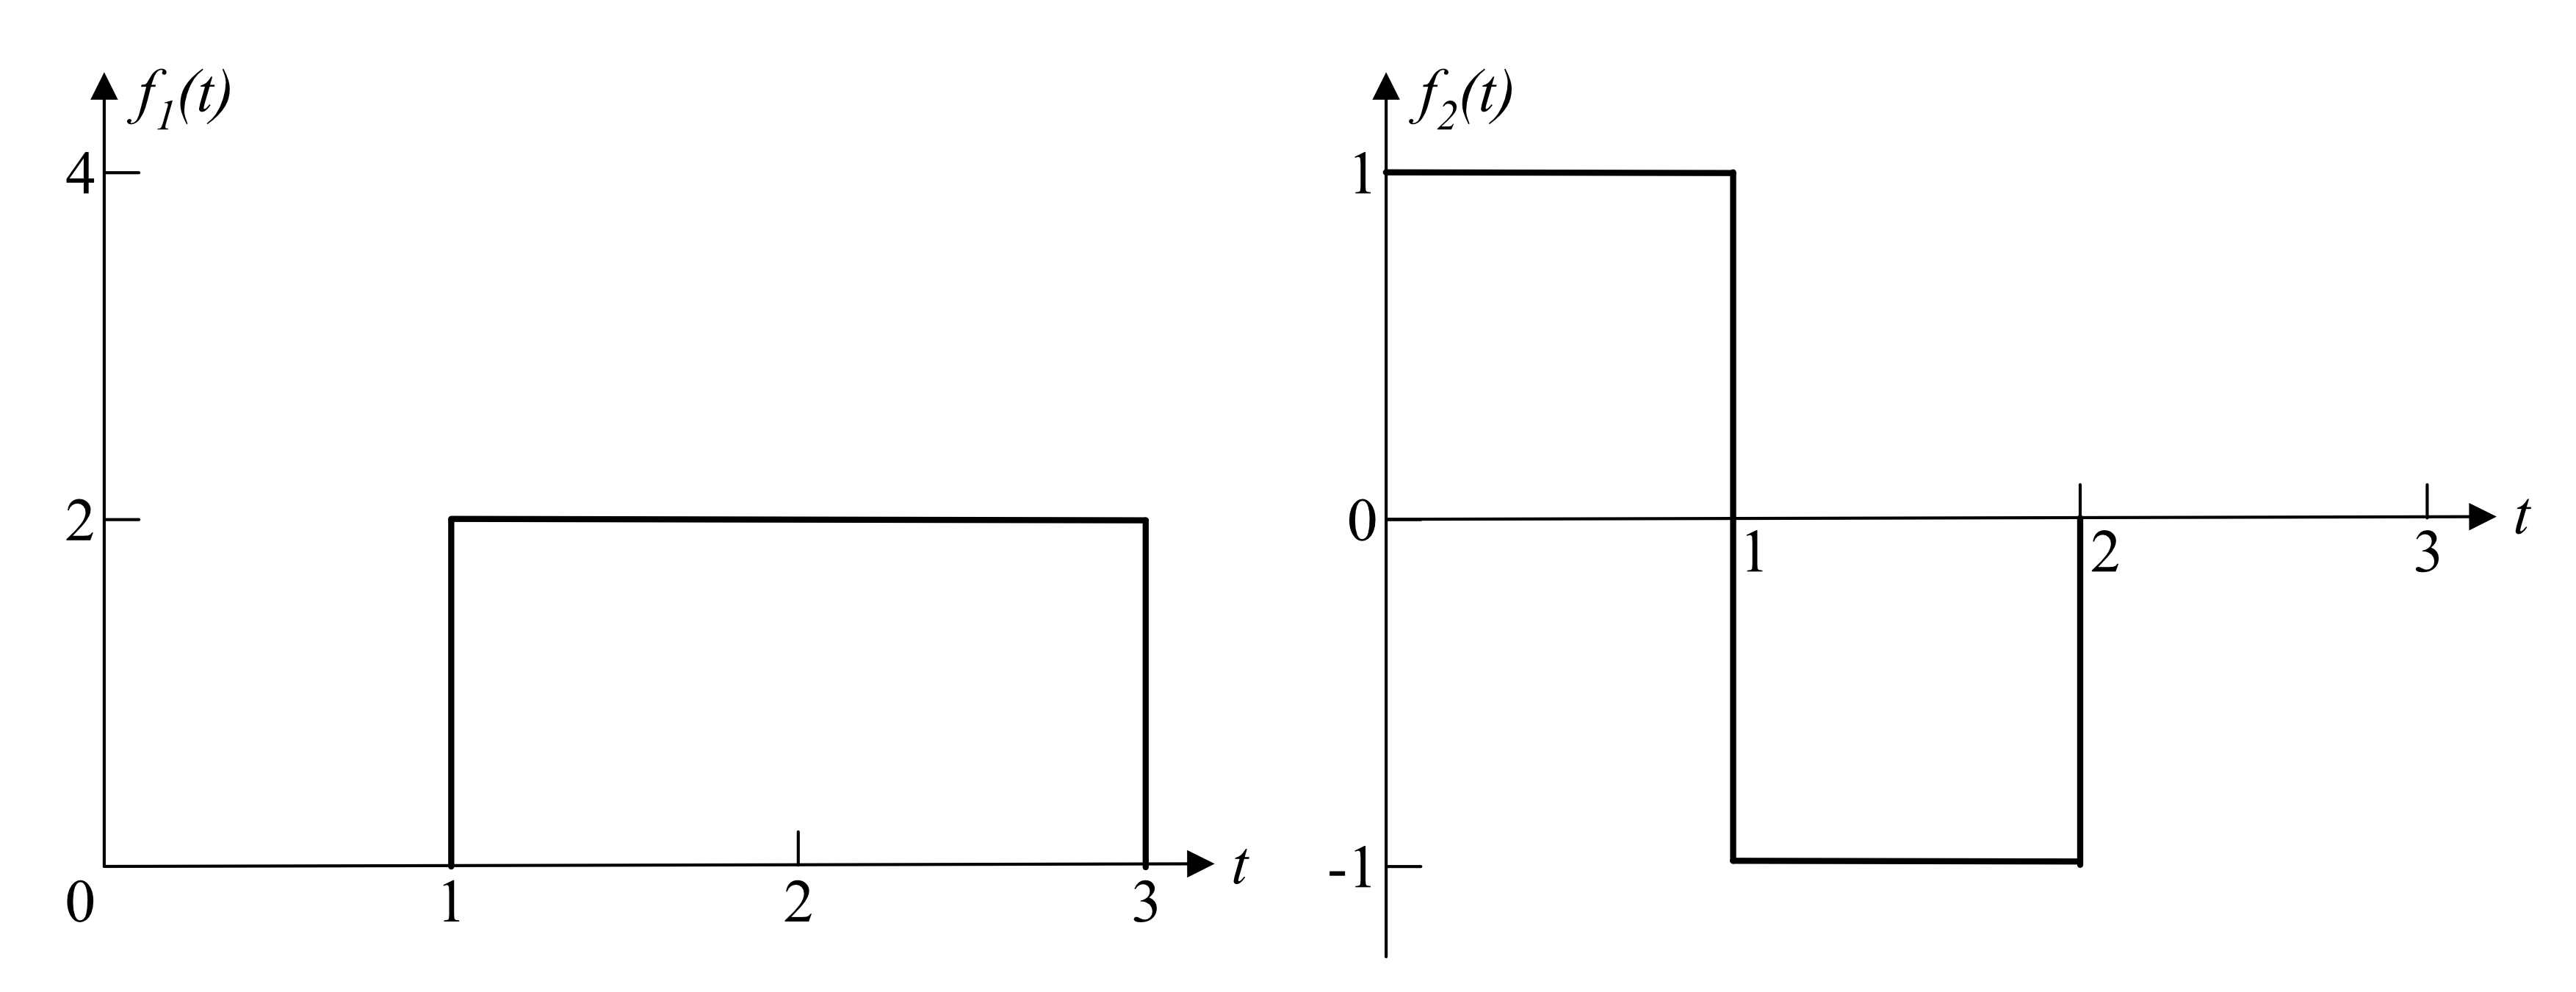
\includegraphics[width=12cm]{assets/hw3img1.png}
			\centering
		\end{figure}
		\quad
	\end{problem}
	
	
\end{document}